\documentclass[11pt]{aghdpl}
% \documentclass[en,11pt]{aghdpl}  % praca w języku angielskim

% Lista wszystkich języków stanowiących języki pozycji bibliograficznych użytych w pracy.
% (Zgodnie z zasadami tworzenia bibliografii każda pozycja powinna zostać utworzona zgodnie z zasadami języka, w którym dana publikacja została napisana.)
\usepackage[english,polish]{babel}

% Użyj polskiego łamania wyrazów (zamiast domyślnego angielskiego).
\usepackage{polski}

\usepackage[utf8]{inputenc}

% dodatkowe pakiety

\usepackage{mathtools}
\usepackage{amsfonts}
\usepackage{amsmath}
\usepackage{amsthm}

% --- < bibliografia > ---

\usepackage[
style=numeric,
sorting=none,
language=autobib,
autolang=other,
urldate=iso8601,
backref=false,
isbn=true,
url=false,
maxbibnames=3,
backend=biber
]{biblatex}

%
% Zastosuj styl wpisu bibliograficznego właściwy językowi publikacji.
%language=autobib,
%autolang=other,
% Zapisuj datę dostępu do strony WWW w formacie RRRR-MM-DD.
%urldate=iso8601,
% Nie dodawaj numerów stron, na których występuje cytowanie.
%backref=false,
% Podawaj ISBN.
%isbn=true,
% Nie podawaj URL-i, o ile nie jest to konieczne.
%url=false,
%
% Ustawienia związane z polskimi normami dla bibliografii.
%maxbibnames=3,
% Jeżeli używamy BibTeXa:
%backend=bibtex
%]{biblatex}

\usepackage{csquotes}
% Ponieważ `csquotes` nie posiada polskiego stylu, można skorzystać z mocno zbliżonego stylu chorwackiego.
\DeclareQuoteAlias{croatian}{polish}

\addbibresource{bibliografia.bib}

% Nie wyświetlaj wybranych pól.
%\AtEveryBibitem{\clearfield{note}}


% ------------------------
% --- < listingi > ---

% Użyj czcionki kroju Courier.
\usepackage{courier}

\usepackage{listings}
\lstloadlanguages{TeX}

\lstset{
	literate={ą}{{\k{a}}}1
           {ć}{{\'c}}1
           {ę}{{\k{e}}}1
           {ó}{{\'o}}1
           {ń}{{\'n}}1
           {ł}{{\l{}}}1
           {ś}{{\'s}}1
           {ź}{{\'z}}1
           {ż}{{\.z}}1
           {Ą}{{\k{A}}}1
           {Ć}{{\'C}}1
           {Ę}{{\k{E}}}1
           {Ó}{{\'O}}1
           {Ń}{{\'N}}1
           {Ł}{{\L{}}}1
           {Ś}{{\'S}}1
           {Ź}{{\'Z}}1
           {Ż}{{\.Z}}1,
	basicstyle=\footnotesize\ttfamily,
}

% ------------------------

\AtBeginDocument{
	\renewcommand{\tablename}{Tabela}
	\renewcommand{\figurename}{Rys.}
}

% ------------------------
% --- < tabele > ---

\usepackage{array}
\usepackage{tabularx}
\usepackage{multirow}
\usepackage{booktabs}
\usepackage{makecell}
\usepackage[flushleft]{threeparttable}

\usepackage{fancyref}

% defines the X column to use m (\parbox[c]) instead of p (`parbox[t]`)
\newcolumntype{C}[1]{>{\hsize=#1\hsize\centering\arraybackslash}X}


%---------------------------------------------------------------------------

\author{Kamil Osuch}
\shortauthor{K. Osuch}

\titlePL{Porównanie budowania i rozwoju aplikacji WWW w języku Elm i~technologiach React+Redux}
\titleEN{Comparision of building and development of web application in Elm language and React+Redux technologies}


\shorttitlePL{Porównanie budowania i rozwoju aplikacji WWW w języku Elm i~technologiach React+Redux} % skrócona wersja tytułu jeśli jest bardzo długi
\shorttitleEN{Comparision of building and development of web application in Elm language and React+Redux technologies}

\thesistype{Praca dyplomowa inżynierska}
%\thesistype{Master of Science Thesis}

\supervisor{dr inż. Piotr Matyasik}
%\supervisor{Marcin Szpyrka PhD, DSc}

\degreeprogramme{Informatyka}
%\degreeprogramme{Computer Science}

\date{2017}

\department{Katedra Informatyki Stosowanej}
%\department{Department of Applied Computer Science}

\faculty{Wydział Elektrotechniki, Automatyki,\protect\\[-1mm] Informatyki i Inżynierii Biomedycznej}
%\faculty{Faculty of Electrical Engineering, Automatics, Computer Science and Biomedical Engineering}

\acknowledgements{Serdecznie dziękuję \dots tu ciąg dalszych podziękowań np. dla promotora, żony, sąsiada itp.}


\setlength{\cftsecnumwidth}{10mm}

%---------------------------------------------------------------------------
\setcounter{secnumdepth}{4}
\brokenpenalty=10000\relax

\begin{document}

\titlepages

% Ponowne zdefiniowanie stylu `plain`, aby usunąć numer strony z pierwszej strony spisu treści i poszczególnych rozdziałów.
\fancypagestyle{plain}
{
	% Usuń nagłówek i stopkę
	\fancyhf{}
	% Usuń linie.
	\renewcommand{\headrulewidth}{0pt}
	\renewcommand{\footrulewidth}{0pt}
}

\setcounter{tocdepth}{2}
\tableofcontents
\clearpage

\chapter{Wprowadzenie} \label{chap:wprowadzenie}

W ciągu ostatnich kilku lat sposób tworzenia stron internetowych przechodził intensywne i szybkie zmiany. W związku z rosnącą popularnością internetu na całym świecie okazało się, że zwykłe, proste strony internetowe nie są wystarczające. W związku z tym szybko one awansowały ze statycznych dokumentów hipertekstowych jedynie wyświetlających zawartość użytkownikowi, do poziomu aplikacji internetowych, z którymi może on wejść w interakcję, a nawet używać ich dokładnie tak samo, jak programów zainstalowanych w swoim systemie operacyjnym. 

Rynek tworzenia oprogramowania webowego został przejęty głównie przez język JavaScript nazywany dziś przez niektórych asemblerem stron internetowych \cite{JSAssembly}. Coraz większe wymagania co do działania stron internetowych spowodowały, że tworzenie stron bezpośrednio w JavaScript'cie stało się zbyt skomplikowane i niewystarczające. Z pomocą przychodzą biblioteki, frameworki oraz języki kompilowane do JavaScriptu. Upraszczają one tworzony kod, często zmieniając też jego strukturę. Dzięki temu umożliwiają korzystanie z gotowych funkcjonalności w prosty i wygodny sposób. Przykładami tutaj mogą być biblioteki takie jak jQuery, Angular, React, Redux, czy Ember.js. 

W przypadku języków kompilowanych do JavaScriptu zmiany są jeszcze większe. Programista nie zastanawia się nad tym, że ostateczna wersja stworzonego przez niego programu jest zapisana w zupełnie innym języku. Przykładami takich języków są chociażby CoffeeScript, TypeScript czy Elm.

Ilość takich rozwiązań tworzy nieograniczoną liczbę podejść do tworzenia aplikacji webowych, a ich liczba każdego dnia rośnie. W związku z tym powstaje wiele artykułów porównujących różne podejścia, zarówno pod względami architektury kodu, jak i szybkości działania samych aplikacji.

Celem niniejszej pracy jest porównanie budowania i rozwoju aplikacji webowych przy pomocy języka Elm, oraz kombinacji bibliotek React.js i Redux. Technologie te zostaną szczegółowo porównane pod względem dostępnych funkcjonalności, szybkości działania aplikacji, dostępności bibliotek oraz trudności zarówno w tworzeniu pierwszej wersji aplikacji, jak i rozwoju istniejącego już kodu.

Wybór tematu pracy był podyktowany przede wszystkim poszukiwaniem alternatywnych rozwiązań służących do tworzenia aplikacji webowych. Biblioteki takie jak React czy Redux zdominowały rynek, przez co ilość wykorzystywanych sposobów budowania stron internetowych w stosunku do ilości dostępnych możliwości jest bardzo mała.

Ważną częścią pracy jest próba implementacji w języku Elm części projektu stworzonego przy pomocy kombinacji Reacta i~Reduxa. Pozwoli to na praktyczną możliwość analizy obu rozwiązań i wyspecyfikowanie napotkanych problemów.

W rozdziale \ref{chap:teoria} zostały krótko opisane charakterystyka języka JavaScript oraz podstawowe pojęcia związane z tworzeniem aplikacji webowych. Następnie krótko zostały opisane biblioteki React i Redux oraz język Elm.
Rozdział \ref{chap:porownanie} skupia się na porównaniu architektury obu rozwiązań, zwracając uwagę zarówno na funkcjonalności, które są dostępne domyślnie jednocześnie Elmie oraz kombinacji Reacta i~Reduxa, jak i na te rozwiązania, które domyślnie oferuje tylko jedna ze stron.
W rozdziale \ref{chap:tools} opisane zostały narzędzia, które są oferowane przez oba porównywane rozwiązania, ich możliwości, ograniczenia, a także poziom trudności ich użycia.
Rozdział \ref{chap:implementacja} opisuje założenia implementacji projektu tworzonego w ramach pracy, oraz problemy napotkane podczas próby stworzenia aplikacji, domyślnie napisanej za pomocą Reacta i Reduxa, przy pomocy języka Elm.
Rozdział \ref{chap:podsumowanie} zawiera krótkie podsumowanie przeprowadzonej analizy porównawczej. Opisuje on wnioski oraz możliwości rozwoju pracy.

\chapter{Podstawy teoretyczne} \label{chap:teoria}
W tym rozdziale zostaną omówione podstawowe pojęcia związane z tematem pracy. Pierwsze dwa podrozdziały skupiają się na opisie czym w ogóle jest aplikacja internetowa, oraz opisują jedno z najpopularniejszych podejść do budowania aplikacji internetowej, SPA. W kolejnych podrozdziałach zostały opisane technologie, które są porównywane w dalszej części pracy.
\section{Aplikacja internetowa}
Aplikacja internetowa jest czymś więcej niż zwykłą stroną internetową. Z definicji jest to aplikacja typu klient-serwer, w której klient jest uruchamiany przy pomocy przeglądarki internetowej. Oprogramowanie klienta jest pobierane na komputer klienta podczas wizyty na odpowiedniej stronie internetowej, przy użyciu standardowych procedur, takich jak HTTP. Aktualizacje oprogramowania klienta mogą odbywać się za każdym razem, gdy odwiedzana jest strona internetowa. W czasie trwania sesji przeglądarka internetowa interpretuje i wyświetla strony, oraz działa jako uniwersalny klient dla dowolnej aplikacji internetowej.
\begin{figure}[h]
	\centering
	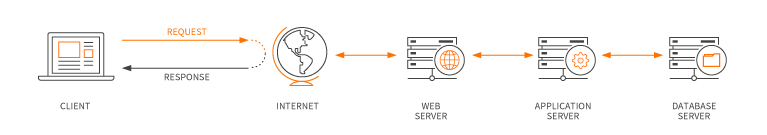
\includegraphics[width=\textwidth]{images/how_web_application_works}
	\caption{Podstawowy schemat działania aplikacji internetowej \cite{MaxCdnWebApp}}
\end{figure}
%\subsection{Krótki rys historyczny}
\section{SPA}Skrót SPA pochodzi od \textit{Single-page Application}. Jest to aplikacja internetowa działająca wewnątrz przeglądarki, która podczas użytkowania strony nie wymaga odświeżania strony. W tym podejściu, cały niezbędny kod źródłowy --- HTML, JavaScript i CSS --- jest pobierany przy pojedyńczym załadowaniu strony, lub odpowiednie zasoby są ładowane dynamicznie i dodawane do strony jedynie wtedy, kiedy jest to potrzebne. Idea jaka stoi za takim rozwiązaniem, to przede wszystkim lepszy, bardziej naturalny user expierience. Użytkownik po wejściu na stronę, nie musi przy każdej interakcji oczekiwać na ponowne załadowanie się strony, czy też jej odświeżanie.


\begin{figure}[!h]
	\centering
	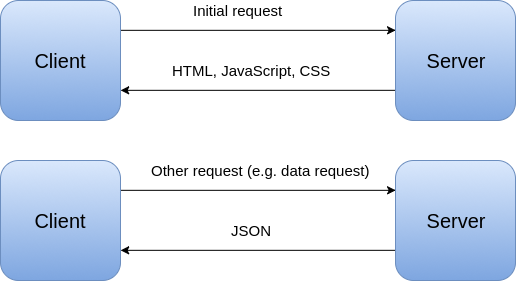
\includegraphics[width=0.6\textwidth]{images/spa}
	\caption{Podstawowy cykl życia SPA}
\end{figure}

Choć koncept SPA zaczął być częściej używany po spopularyzowaniu AJAX'a\footnote{Asynchronous JavaScript And XML}, to tak naprawdę dopiero od kilku lat jest on powszechnie wykorzystywany podczas budowania aplikacji internetowych. Serwisy takie jak Gmail, Google Maps, Twitter czy GitHub są właśnie aplikacjami typu single-page application. Także większość najpopularniejszych bibliotek JavaScript'owych umożliwiają implementację aplikacji internetowej zgodnie z zasadami SPA.
\subsection{Zalety}
\begin{itemize}
	\item Szybkość działania -- większość zasobów jest ładowana tylko raz podczas cyklu życia aplikacji, jedynymi informacjami, które są wymieniane z serwerem cały czas, są dane
	\item Brak ciągłego przeładowywania strony
	\item Znacznie prostszy proces wdrożenia aplikacji -- jedyne co jest potrzebne to statyczny serwer serwujący minimalnie 3 pliki -- pojedynczą stronę HTML, oraz 2 pakiety: jeden zawierający wszystkie style, drugi skupiający w sobie cały kod JavaScriptu
	\item Odciążenie strony serwerowej -- serwer, zamiast generować za każdym razem pełny kod strony, transmituje jedynie potrzebne w danej chwili dane
\end{itemize}
\subsection{Wady}
\begin{itemize}
	\item Powolne początkowe uruchomienie strony -- wymaga ono załadowania frameworku, oraz przynajmniej części aplikacji, która później już nie jest ponownie ściągana.
	\item Ze względu na zależność SPA od JavaScriptu, bardzo łatwo o pojawienie się wycieków pamięci pomiędzy długimi okresami czasu między przeładowaniami strony
\end{itemize}

\section{JavaScript}
JavaScript jest to wysokopoziomowy, słabo typowany, wieloparadgymatowy, skryptowy i interpretowany język programowania stworzony w 1995 roku przez Brendana Eicha dla firmy Netscape.  W roku 1997 organizacja Ecma International wydała na podstawie JavaScriptu standard języka skryptowego nazwany ECMAScript, na którym bazowanych jest większość silników JavaScript'owych.

JavaScript jest jedną z trzech głównych technologii wykorzystywanych przy tworzeniu treści związanych z siecią internetową. Obecnie 94,9\% spośród 10 milionów najbardziej popularnych stron internetowych wykorzystuje JavaScript (stan na grudzień 2017 \cite{JSUsage}).

\section{React.js}
React jest biblioteką języka JavaScript, wykorzystywaną do tworzenia graficznych interfejsów użytkownika. Pozwala ona na tworzenie rozbudowanych aplikacji internetowych, które używają danych i~mogą zmieniać swoją zawartość w czasie bez ponownego ładowania strony. Biblioteka została stworzona przez jednego z programistów Facebooka, Jordana Walke, który zainspirował się rozszerzeniem języka PHP, XHP, także stworzonym przez Facebooka. Pierwsze wersje biblioteki zostały użyte w 2011 roku na stronie aktualności Facebooka, a od 2012 roku jest ona wykorzystywana w~serwisie Instagram. Od 2013 roku React stał się wolnym oprogramowaniem, co spowodowało nagły wzrost jego popularności, a także umożliwiło społeczności  pomoc w rozwoju oprogramowania.

Ze względu na ogromny wpływ rynku urządzeń mobilnych, Facebook ogłosił w 2015 roku bibliotekę React Native, pozwalającą na korzystanie z architektury Reacta podczas budowania aplikacji mobilnych. To co wyróżniało tę bibliotekę od dotychczasowych sposobów tworzenia mobilnego oprogramowania, to brak konieczności powielania funkcjonalności dla każdej platformy z osobna. React Native pozwalał na wykorzystanie tego samego kodu źródłowego zarówno w aplikacji dla systemu Android jak i iOS.

Obecnie React jest jedną z najpopularniejszych bibliotek służących do tworzenia aplikacji internetowych. Jest wykorzystywany w ogromnej ilości znanych serwisów takich jak Facebook, Instagram, Spotify, Netflix czy eBay. 
\section{Redux}
Redux jest biblioteką języka JavaScript o otwartym kodzie źródłowym zaprojektowaną do zarządzania stanem aplikacji. Została stworzona w 2015 roku przez Dana Abramova. Działanie Reduxa może być opisane przez trzy zasady \cite{reduxDocs}:
\begin{enumerate}
	\item Istnieje jedno źródło prawdy -- stan całej aplikacji jest przechowywany w pojedyńczym obiekcie, który przechowuje całe drzewo stanu aplikacji.
	\item Stan służy tylko do odczytu -- jedynym sposobem na zmianę stanu jest wysłanie akcji -- obiektu opisującego co się stało, zwykle zawierającego typ akcji, oraz ewentualne dane, które mają wpływ na zmianę stanu.
	\item Zmiany stanu są dokonywane przy użyciu czystych funkcji -- aby określić, w jaki sposób drzewo stanu jest modyfikowane przez akcje, tworzy się funkcje zwane \textit{reducerami}, przyjmujące poprzedni stan i akcję jako argumenty, a zwracające nowy stan.
\end{enumerate}
\begin{figure}[h]
	\centering
	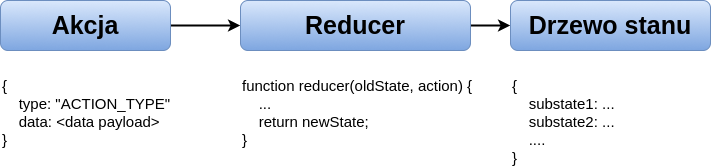
\includegraphics[width=0.9\textwidth]{images/redux_flow}
	\caption{Schemat działania Reduxa}
\end{figure}

\section{Elm}
Elm jest funcyjnym językiem programowania kompilowanym do JavaScriptu. Język został stworzony w 2012 roku przez Evana Czaplickiego, w ramach jego pracy dyplomowej. Na dalszy rozwój języka pozwoliła firma Prezi, która w 2013 roku zatrudniła twórcę języka. W 2016 roku Czaplicki zmienił firmę na NoRedInk i postanowił stworzyć organizację non-profit --- Elm Software Foundation --- której celem ma być promowanie, ochrona i rozwój języka Elm, oraz wszelka pomoc społeczności programistów tworzących oprogramowanie w Elmie \cite{newAdventures}.

Evan Czaplicki twierdzi, że jego język może konkurować z projektami takimi jak React, jako narzędzie do tworzenia aplikacji internetowych. Język kładzie bardzo duży nacisk na prostotę, łatwość użycia i jakość narzędzi \cite{elmGuide}.
\chapter{Podsumowanie} \label{chap:podsumowanie}
Celem tej pracy było porównanie dwóch sposobów budowania i rozwoju aplikacji internetowych: przy pomocy języka Elm oraz kombinacji bibliotek React.js i Redux. 
Obie technologie miały zostać porównane pod względem architektury, udostępnianych funkcjonalności, wydajności aplikacji oraz dostępnych bibliotek i narzędzi. Dodatkowo w ramach praktycznego porównania miała zostać przygotowana aplikacja stworzona przy pomocy języka Elm, która odwzorowywała pewną część innej aplikacji napisanej przy pomocy bibliotek React i Redux. 

Pomimo porównania języka do dwóch bibliotek, okazało się, że pod względem architektonicznym połączenie Reacta i Reduxa jest bardzo podobne do podejścia stosowanego w języku Elm. Te same funkcjonalności zaimplementowane w różny sposób pozwoliły na porównanie, która z technologii może być oceniana jako lepsza w kontekście tworzenia aplikacji internetowych. Sporym czynnikiem mającym wpływ na ocenę obu technologii były problemy, które pojawiły się podczas realizacji praktycznej części pracy w formie projektu. 

Analiza architektury języka Elm oraz bibliotek React i Redux pokazała, że w zależności od wybranego kontekstu, na podstawie którego te technologie są porównywane, decyzja o tym, która z nich jest lepsza, potrafi być zmienna. 

Pod względem szybkości wyświetlania widoku zdecydowanym zwycięzcą jest Elm, który dzięki optymalizacjom zawartym w swoim silniku do budowy Virtual DOM-u jest w stanie pominąć niektóre klatki, które i tak nie są widoczne dla użytkownika. Argumentem stojącym za wyborem Elma jest też to, że pewne elementy, takie jak narzędzia do analizy kodu i procesu działania aplikacji są wbudowane bezpośrednio w sam silnik języka, w przeciwieństwie do Reacta i Reduxa, które muszą korzystać z zewnętrznych rozwiązań, o których trzeba pamiętać. Część porównywanych elementów architektury nie pozwala jednak na bezpośrednie wybranie lepszej technologii, ponieważ każdy programista preferuje inne podejście do tworzenia oprogramowania. Mowa tu o elementach takich jak wybór między silnym a~dynamicznym typowaniem, preferencji trzymania wszystkich danych w jednym miejscu, a możliwością skorzystania z lokalnego stanu oferowanego przez komponenty, czy chociażby wybór między komponentami zawierającymi własny cykl życia a funkcjami w Elmie działającymi za każdym razem w ten sam sposób, bez efektów ubocznych. Aspektem, który stawia Reacta i Reduxa na wygranej pozycji jest przede wszystkim ich popularność oraz dostępność bibliotek. Z racji tego, że są to po prostu biblioteki języka JavaScript, mogą one korzystać bezpośrednio z każdego dostępnego pakietu stworzonego przy pomocy tego języka, który jest obecnie najpopularniejszym językiem do budowania aplikacji internetowych.

Podsumowując całą pracę, nie można wybrać, która z porównywanych technologii jest lepsza. Zarówno język Elm, jak i kombinacja Reacta i Reduxa mają swoje zalety, a także wady. Trzeba zwrócić także uwagę na to, że porównując technologie wykorzystywane do tworzenia aplikacji internetowych, wyników takiego porównania nie można brać pod uwagę przez dłuższy okres. Rynek tworzenia oprogramowania webowego jest jednym z najczęściej i najszybciej zmieniających się gałęzi programowania. Być może za kilka lat zmieni się on na tyle, że jego popularność wzrośnie i całkowicie wyprze używane obecnie biblioteki. 



% itd.
% \appendix
% \include{dodatekA}
% \include{dodatekB}
% itd.
\printbibliography

\end{document}
